Recently, cryptocurrencies such as Bitcoin, Ether, and Dogecoin have gained increasing attention from traders and investors. In particular, the first cryptocurrency called Bitcoin - developed by an unknown individual or group under the pseudonym Satoshi Nakamoto and first presented in 2009 \cite{Bitcoin2009} - has achieved a market cap of about $750$ billion United States dollar (USD) as of \date{14 June 2021}. This is comparable to the market cap of companies like Facebook and Tesla at the stock market \cite{MarketCapCompany2021}\cite{MarketCapBitcoin2021}.\\

The original purpose of Bitcoin is the establishment of a form of decentralized digital money that can be used for uncensored transactions on the internet. The basis of Bitcoin is the so-called blockchain. As its name suggests, the blockchain is an ordered chain of blocks. Each block contains Bitcoin transactions from a certain time period (typically, roughly $10$ minutes). New blocks - and thus new recorded transactions - are appended to the blockchain by solving a mathematical task. The task is solved by investing computing power. The person or entity that solves the mathematical task first is rewarded with new Bitcoins and with the transactions fees of all transactions in the new block. The addition of a new block to the blockchain and the distribution of new Bitcoins is called Bitcoin mining. A simplified illustration of the Bitcoin blockchain is depicted in Fig.~\ref{fig:blockchain}.

\begin{figure}[h!]
  \centering
  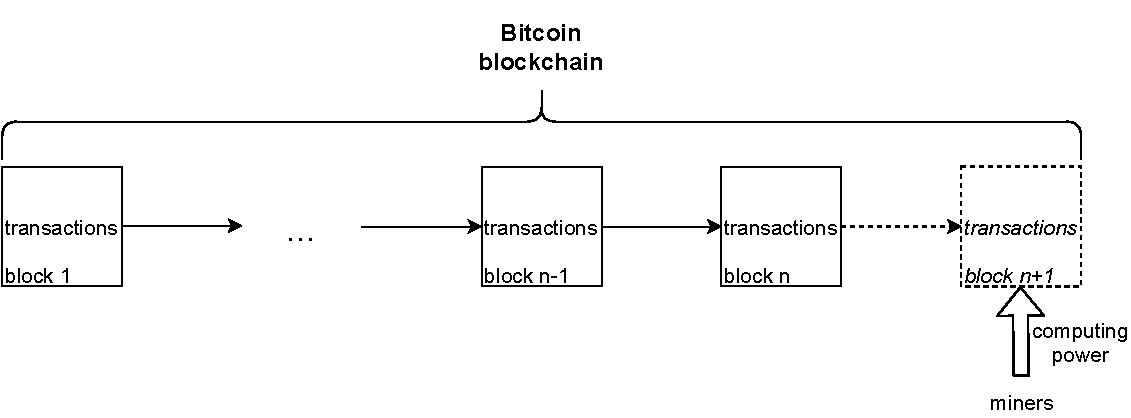
\includegraphics[width=\textwidth]{bitcoin_blockchain.pdf}
  \caption{Simplified illustration of the Bitcoin blockchain starting from the first block nr. $1$ that is also called genesis block, and was mined by Satoshi Nakamoto in 2009. Each block contains information on Bitcoin transactions for time periods of roughly $10$ minutes. Suppose, the current length of the Bitcoin blockchain is given by $n$ blocks. The addition of a new block with the nr. $n+1$ to the blockchain is called Bitcoin mining, and is achieved by investing computing power in solving a mathematical task.}
  \label{fig:blockchain}
\end{figure}

Besides its original intention of a form of digital money, Bitcoins are more and more treated as a financial asset that is exchanged at specific exchanges. These exchanges are called cryptocurrency exchanges because they allow their customers to exchange Bitcoin with other cryptocurrencies and with fiat currencies such as USD. Examples for cryptocurrency exchanges are Binance, Kraken, and Coinbase. As a financial asset, the Bitcoin market price is the result of demand and supply that is limited as the distribution of new Bitcoins requires computing power. This makes the Bitcoin comparable to classical financial assets such as company shares. However, its volatility is usually much larger than share prices at the stock market \cite{bitcoin_book_2018}. \\

For traders and investors, it is of course of interest to predict the future development of Bitcoin's market price in order to maximize returns. The present work is concerned with the prediction of tomorrow's market price based on data from today and the past days. The prediction of the Bitcoin market price is treated as a binary classification problem, such that predictions are either \enquote{up} or \enquote{down}, dependent on the predicted direction of tomorrow's Bitcoin market price.\\

The structure of the present paper is as follows. In Section~\ref{sec:dataset}, time series data of the Bitcoin market price and other measures are transformed into a dataset that is suitable for a binary classification task as described above. The binary classification dataset allows the application of supervised machine learning algorithms, whose theoretical basics are summarized in Section~\ref{sec:theory}. In addition, the same Section includes an explanation on techniques that are applied to optimize hyperparameters and to evaluate the performance of these machine learning algorithms. Section~\ref{sec:implementation_software} contains a list of the software that is applied to develop the binary classification dataset and to implement the prediction algorithms. The results of the application of the different machine learning algorithms on the Bitcoin price development classification problem are presented in Section~\ref{sec:results}. A comparison of the different learning algorithms as well as a detailed discussion of the results is given in Section~\ref{sec:discussion}. Finally, in Section~\ref{sec:conclusion_outlook}, the findings of the present work are summarized.